Dada la siguiente topología:
  \begin{figure}[h]
    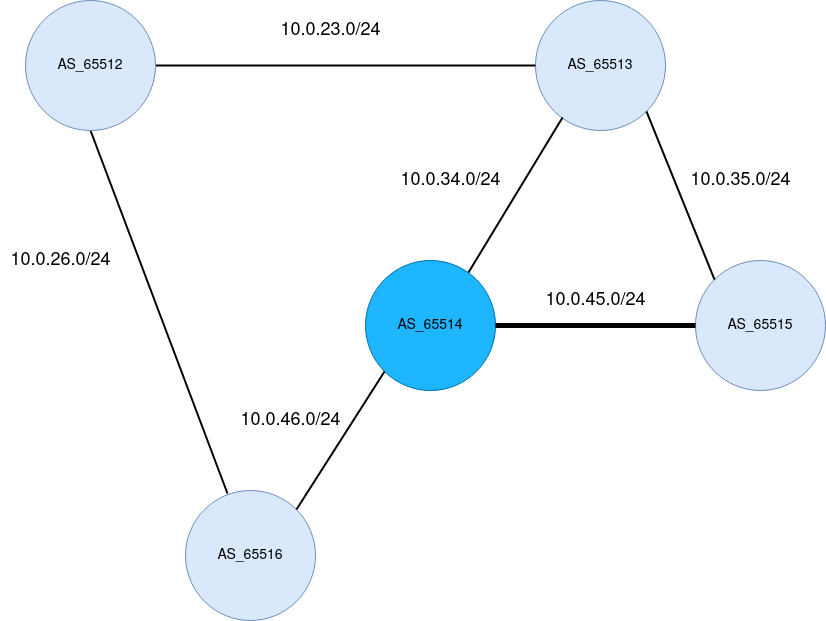
\includegraphics[width=\textwidth]{route-map.png}
  \end{figure}

  \begin{itemize}
    \item El AS65514 desea usar preferentemente su enlace con AS65515,
    y mantener los otros dos como respaldo (backup)
    \item Implementar esa política mediante el uso de \texttt{route-map} .
  \end{itemize}

  Detalles a tener en cuenta:

  \begin{itemize}
    \item Redes de usuario:
    \begin{itemize}
      \item IPv4: 172.16.X.0/24
      \item IPv6: 2001:db8:X::/64
    \end{itemize}
  \end{itemize}

  \[ \forall X \in \{12,13,14,15,16\} \]


  \begin{minted}{bash}
    # net.conf
    defsw br23 uml2.0 uml3.0
    defsw br34 uml3.1 uml4.0
    defsw br35 uml3.2 uml5.0
    defsw br45 uml4.1 uml5.1
    defsw br26 uml2.1 uml6.0
    defsw br46 uml4.2 uml6.1
  \end{minted}

  \begin{minted}{bash}
    # En cuanto se inician las UML, editar el fichero /etc/quagga/daemons la línea
    bgpd=no
    # Por
    bgpd=yes
    # A continuación restart del servicio
    systemctl restart quagga
    # Verificar que se bgpd está corriendo
    systemctl status quagga
  \end{minted}

  \begin{minted}{lexer.py:IOSLexer -x}
    ! UML2 (zebra.conf)
    con[figure] t[erminal]
    int[erface] eth0
    ip addr 10.0.23.1/24
    no s[hutdown]
    q[uit]
    int[erface] eth1
    ip addr 10.0.26.1/24
    no s[hutdown]
    quit
    ip f[orwarding]
    write
  \end{minted}

  \begin{minted}{lexer.py:IOSLexer -x}
    ! UML3 (zebra.conf)
    con[figure] t[erminal]
    int[erface] eth0
    ip address 10.0.23.2/24
    no s[hutdown]
    q[uit]
    int[erface] eth1
    ip address 10.0.34.1/24
    no s[hutdown]
    q[uit]
    int[erface] eth2
    ip address 10.0.35.1/24
    no s[hutdown]
    q[uit]
    ip f[orwarding]
    write
  \end{minted}

  \begin{minted}{lexer.py:IOSLexer -x}
    ! UML4 (zebra.conf)
    con[figure] t[erminal]
    int[erface] eth0
    ip address 10.0.34.2/24
    no s[hutdown]
    q[uit]
    int[erface] eth1
    ip address 10.0.45.1/24
    no s[hutdown]
    q[uit]
    int[erface] eth2
    ip address 10.0.46.1/24
    no s[hutdown]
    q[uit]
    ip f[orwarding]
    write
  \end{minted}

  \begin{minted}{lexer.py:IOSLexer -x}
    ! UML5 (zebra.conf)
    con[figure] t[erminal]
    int[erface] eth0
    ip address 10.0.35.2/24
    no s[hutdown]
    q[uit]
    int[erface] eth1
    ip address 10.0.45.2/24
    no s[hutdown]
    q[uit]
    ip f[orwarding]
    write
  \end{minted}

  \begin{minted}{lexer.py:IOSLexer -x}
    ! UML6 (zebra.conf)
    con[figure] t[erminal]
    int[erface] eth0
    ip address 10.0.26.2/24
    int[erface] eth1
    ip address 10.0.46.2/24
    no s[hutdown]
    q[uit]
    ip f[orwarding]
    write
  \end{minted}

  \begin{minted}{lexer.py:IOSLexer -x}
    ! UML2 (bgpd.conf)
    con[figure] t[erminal]
    router bgp 65512
      bgp router-id 10.0.26.1
      ! La red pública que se anuncia en los mensajes BGP que se intercambian
      network 172.16.2.0/24
      ! Establecimiento de los vecinos
      neighbor 10.0.23.2 remote-as 65513
      neighbor 10.0.26.2 remote-as 65516
      ! To enter address family configuration mode for configuring routing sessions,
      ! such as BGP, that use standard IPv6 address prefixes,
      ! use the address-family ipv6 command in router configuration mode
      address-family ipv6
      ! La red IPv4 que se anuncia en los mensajes BGP que se intercambian
      network 2001:db8:2::/64
      neighbor 10.0.23.2 activate
      neighbor 10.0.26.2 activate
      exit-address-family
      do w[rite]
  \end{minted}

  \begin{minted}{lexer.py:IOSLexer -x}
    ! UML3 (bgpd.conf)
    con[figure] t[erminal]
    router bgp 65513
      bgp router-id 10.0.35.1
      network 172.16.3.0/24
      neighbor 10.0.23.1 remote-as 65512
      neighbor 10.0.34.2 remote-as 65514
      neighbor 10.0.35.2 remote-as 65515
      address-family ipv6
      network 2001:db8:3::/64
      neighbor 10.0.23.1 activate
      neighbor 10.0.34.2 activate
      neighbor 10.0.35.2 activate
      exit-address-family
      do w[rite]
  \end{minted}

  \begin{minted}{lexer.py:IOSLexer -x}
    ! UML4 (bgpd.conf)
    con[figure] t[erminal]
    router bgp 65514
      bgp router-id 10.0.46.1
      network 172.16.4.0/24
      neighbor 10.0.34.1 remote-as 65513
      ! Añade una politica de route-map de salida
      neighbor 10.0.34.1 route-map backup out
      neighbor 10.0.45.2 remote-as 65515
      ! Añade una politica de route-map de entrada
      neighbor 10.0.45.2 route-map preferente in
      neighbor 10.0.46.2 remote-as 65516
      ! Añade una politica de route-map de salida
      neighbor 10.0.46.2 route-map backup out
    !
      address-family ipv6
      network 2001:db8:4::/64
      neighbor 10.0.34.1 activate
      neighbor 10.0.45.2 activate
      neighbor 10.0.46.2 activate
      exit-address-family
    !
      route-map preferente permit 10
      ! Establece un local-preference para
      ! que la ruta tenga mayor preferencia que otra
      set local-preference 200
    !
      route-map backup permit 10
      ! Realiza un prepend del identificador
      ! para asegurar que la ruta tiene menor
      ! preferencia que la anterior
      set as-path prepend 65514 65514 65514 65514 65514 65514 65514
    !
      do w[rite]
  \end{minted}

  \begin{minted}{lexer.py:IOSLexer -x}
    ! UML5 (bgpd.conf)
    con[figure] t[erminal]
    router bgp 65515
      bgp router-id 10.0.35.2
      network 172.16.5.0/24
      neighbor 10.0.35.1 remote-as 65513
      neighbor 10.0.45.1 remote-as 65514
    !
      address-family ipv6
      network 2001:db8:5::/64
      neighbor 10.0.35.1 activate
      neighbor 10.0.45.1 activate
      exit-address-family
    !
      do w[rite]
  \end{minted}

  \begin{minted}{lexer.py:IOSLexer -x}
    ! UML6 (bgpd.conf)
    con[figure] t[erminal]
    router bgp 65516
      bgp router-id 10.0.46.2
      network 172.16.6.0/24
      neighbor 10.0.26.1 remote-as 65512
      neighbor 10.0.46.1 remote-as 65514
    !
      address-family ipv6
      network 2001:db8:6::/64
      neighbor 10.0.26.1 activate
      neighbor 10.0.46.1 activate
      exit-address-family
    !
      do w[rite]
  \end{minted}

  Pruebas:
  \begin{minted}{lexer.py:IOSLexer -x}
    ! En una UML
    clear bgp * ! se borra toda la información BGP de las tablas de todos los routeres
    ! En cada uno de los nodos
    ! Comprobar que pasar por el AS 65514 tiene un sobrecoste adicional por el prepend
    sh[ow] ip bgp
  \end{minted}